\subsection{React: Eine JavaScript Bibliothek zum Erstellen von Benutzeroberflächen}
\cite{reactjs}
\label{reactjs}


\begin{figure*}[H]
  \subfigure[Rick and Morty Staffel 1 Werbebild~\cite{rickAndMortySeason1}]{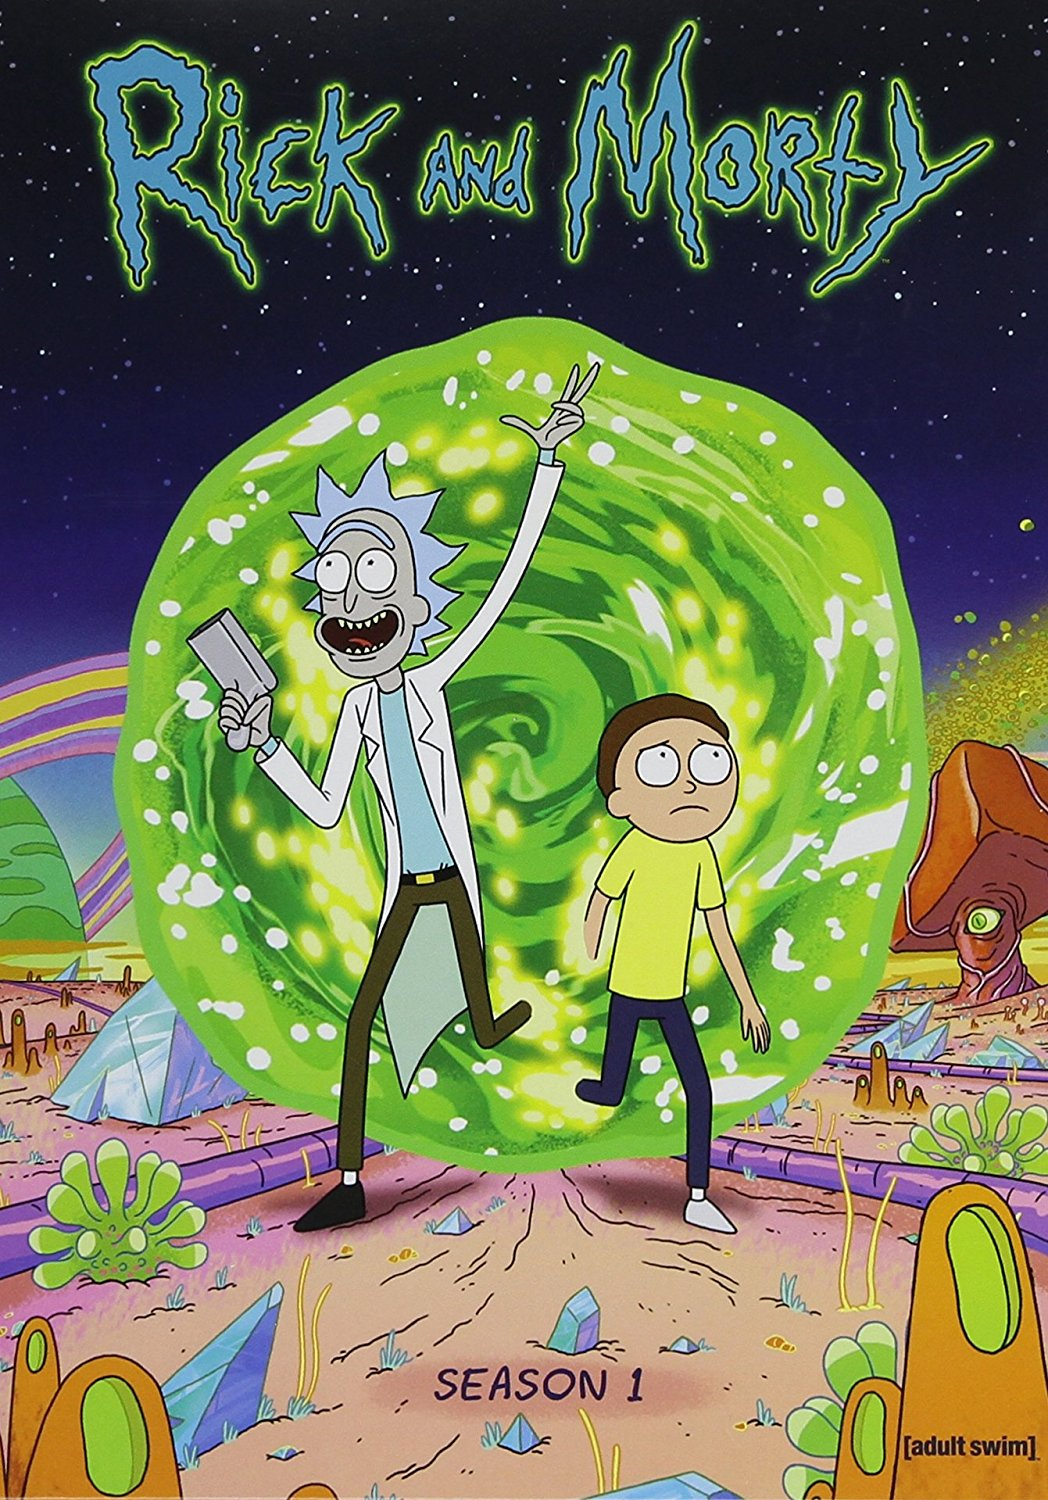
\includegraphics[height=0.4\textwidth]{images/Intro/RnM_S1.jpg}}
\end{figure*}

\begin{figure}[H]
  \begin{center}
    
\includegraphics[width=0.65\textwidth]{Theorie/React/React-icon.svg.png}
    \caption{ReactJS Logo \cite{reactjs}}
  \end{center}
\end{figure}


